\frame
{
\frametitle{\oran{Finanzas Computacionales}}

Nuestro centro provee soluciones computacionales financieras a nivel nacional e
internacional.

Proyectos:


\begin{columns}
\column{0.4\textwidth}
\begin{itemize}
\item Diseño e implementación de algoritmos para predicción de indicadores financieros que manejan grandes volúmenes de datos y requieren respuestas en micro segundos. 

Empresa: Pan Alpha Trading, Wall Street, New York.
\end{itemize}
\column{0.6\textwidth}
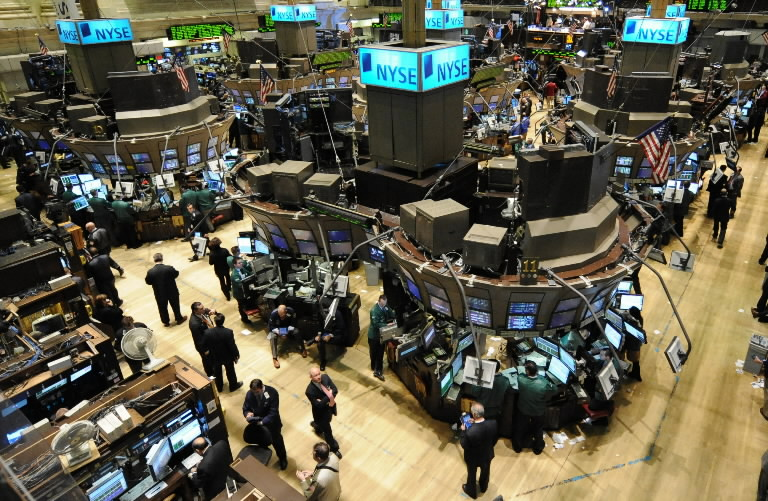
\includegraphics[width=0.7\textwidth]{img/wallstreet}
%\pgfuseimage{wallstreet}
\end{columns}

}

\frame
{
\frametitle{\oran{Finanzas Computacionales}}

\begin{itemize}
\item Desarrollo de aplicación que permite la creación y edición de índices financieros, usando información actualizada diariamente, gran cantidad de activos y data histórica.
\end{itemize}
\begin{center}
 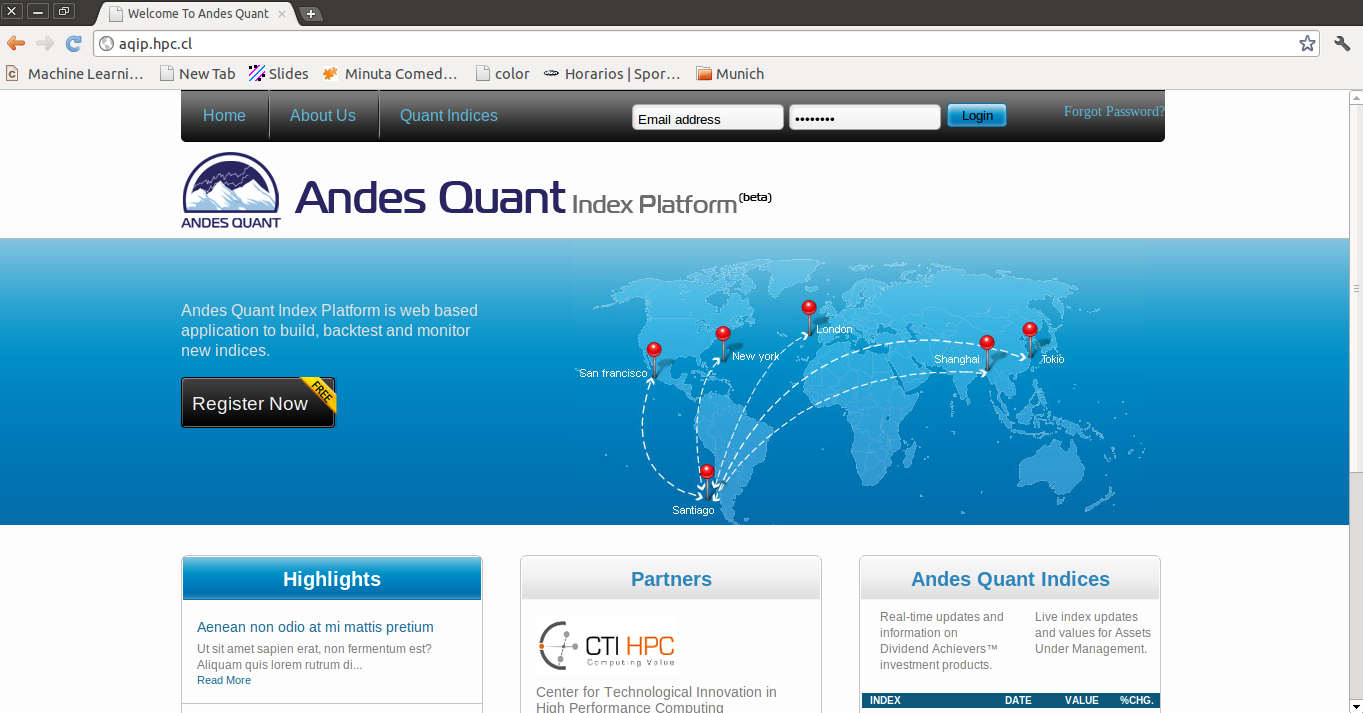
\includegraphics[width=0.7\textwidth]{img/ETF}
\end{center}





}

